\documentclass[journal]{vgtc}                % final (journal style)
%\documentclass[review,journal]{vgtc}         % review (journal style)
%\documentclass[widereview]{vgtc}             % wide-spaced review
%\documentclass[preprint,journal]{vgtc}       % preprint (journal style)
%\documentclass[electronic,journal]{vgtc}     % electronic version, journal

%% Uncomment one of the lines above depending on where your paper is
%% in the conference process. ``review'' and ``widereview'' are for review
%% submission, ``preprint'' is for pre-publication, and the final version
%% doesn't use a specific qualifier. Further, ``electronic'' includes
%% hyperreferences for more convenient online viewing.

%% Please use one of the ``review'' options in combination with the
%% assigned online id (see below) ONLY if your paper uses a double blind
%% review process. Some conferences, like IEEE Vis and InfoVis, have NOT
%% in the past.

%% Please note that the use of figures other than the optional teaser is not permitted on the first page
%% of the journal version.  Figures should begin on the second page and be
%% in CMYK or Grey scale format, otherwise, colour shifting may occur
%% during the printing process.  Papers submitted with figures other than the optional teaser on the
%% first page will be refused.

%% These three lines bring in essential packages: ``mathptmx'' for Type 1
%% typefaces, ``graphicx'' for inclusion of EPS figures. and ``times''
%% for proper handling of the times font family.

\usepackage{mathptmx}
\usepackage{graphicx}
\usepackage{times}

%%% Algorithm packages added by J.P. (not in original template)
\usepackage{algorithm}
\usepackage[noend]{algpseudocode} % algorithm environment

%% We encourage the use of mathptmx for consistent usage of times font
%% throughout the proceedings. However, if you encounter conflicts
%% with other math-related packages, you may want to disable it.

%% This turns references into clickable hyperlinks.
\usepackage[bookmarks,backref=true,linkcolor=black]{hyperref} %,colorlinks
\hypersetup{
  pdfauthor = {},
  pdftitle = {},
  pdfsubject = {},
  pdfkeywords = {},
  colorlinks=true,
  linkcolor= black,
  citecolor= black,
  pageanchor=true,
  urlcolor = black,
  plainpages = false,
  linktocpage
}

%% If you are submitting a paper to a conference for review with a double
%% blind reviewing process, please replace the value ``0'' below with your
%% OnlineID. Otherwise, you may safely leave it at ``0''.
\onlineid{0}

%% declare the category of your paper, only shown in review mode
\vgtccategory{Research}

%% allow for this line if you want the electronic option to work properly
\vgtcinsertpkg

%% In preprint mode you may define your own headline.
%\preprinttext{To appear in an IEEE VGTC sponsored conference.}

%% Paper title.

\title{Subvolume Blocking with Direct Volume Rendering}

%% This is how authors are specified in the journal style

%% indicate IEEE Member or Student Member in form indicated below
\author{Jim Pelton}
\authorfooter{
%% insert punctuation at end of each item
\item
 Jim Pelton is with Boise State University. E-mail: jimpelton@boisestate.edu.
%\item
% Ed Grimley is with Grimley Widgets, Inc.. E-mail: ed.grimley@aol.com.
%\item
% Martha Stewart is with Martha Stewart Enterprises at Microsoft
% Research. E-mail: martha.stewart@marthastewart.com.
}

%other entries to be set up for journal
\shortauthortitle{Pelton \MakeLowercase{\textit{et al.}}: Subvolume Blocking with Direct Volume Rendering}
%\shortauthortitle{Firstauthor \MakeLowercase{\textit{et al.}}: Paper Title}

%% Abstract section.
\abstract{Direct volume rendering (DVR) is a visualization technique for the display of
	3D scalar fields. It excels at rendering interior views of 3D scanned
	objects, simulation data, or any subject lacking a well defined structure, such
	as gaseous phenomena. However, a significant problem with DVR is that the
	memory requirements of volume data sets quickly exceed the size of available
	memory on the graphics processor.  When data exceeds available gpu memory, 
	interactive visualization becomes impossible without using complex out-of-core 
	rendering methods. The problem addressed by this project is that these real-world data sets are
	too large to fit in the largest GPU memory capacities available today
	(12--16GB).  Rendering these volumes requires complicated out-of-core methods that can
	negatively impact visual quality and interactivity.  
} % end of abstract

%% Keywords that describe your work. Will show as 'Index Terms' in journal
%% please capitalize first letter and insert punctuation after last keyword
\keywords{Radiosity, global illumination, constant time}

%% ACM Computing Classification System (CCS). 
%% See <http://www.acm.org/class/1998/> for details.
%% The ``\CCScat'' command takes four arguments.

\CCScatlist{ % not used in journal version
 \CCScat{K.6.1}{Management of Computing and Information Systems}%
{Project and People Management}{Life Cycle};
 \CCScat{K.7.m}{The Computing Profession}{Miscellaneous}{Ethics}
}

%% Uncomment below to include a teaser figure.
%  \teaser{
% \centering
% 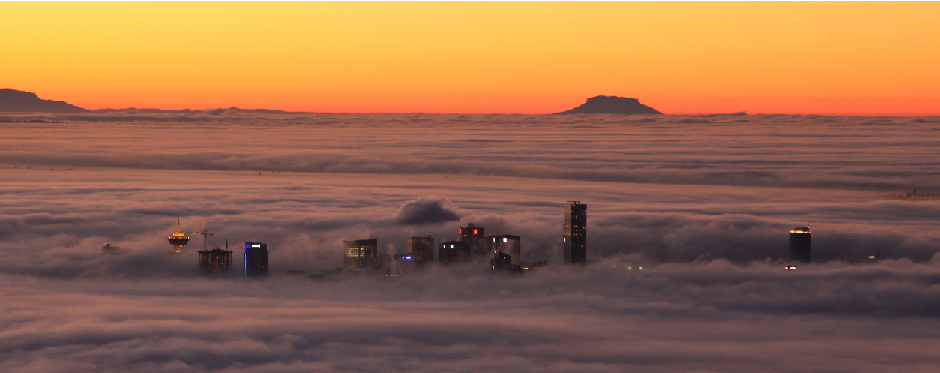
\includegraphics[width=16cm]{CypressView}
%  \caption{In the Clouds: Vancouver from Cypress Mountain.}
%  }

%% Uncomment below to disable the manuscript note
%\renewcommand{\manuscriptnotetxt}{}

%% Copyright space is enabled by default as required by guidelines.
%% It is disabled by the 'review' option or via the following command:
% \nocopyrightspace

%%%%%%%%%%%%%%%%%%%%%%%%%%%%%%%%%%%%%%%%%%%%%%%%%%%%%%%%%%%%%%%%
%%%%%%%%%%%%%%%%%%%%%% START OF THE PAPER %%%%%%%%%%%%%%%%%%%%%%
%%%%%%%%%%%%%%%%%%%%%%%%%%%%%%%%%%%%%%%%%%%%%%%%%%%%%%%%%%%%%%%%%

\begin{document}

%% The ``\maketitle'' command must be the first command after the
%% ``\begin{document}'' command. It prepares and prints the title block.

%% the only exception to this rule is the \firstsection command
\firstsection{Introduction}

\maketitle

%% \section{Introducction} %for journal use above \firstsection{..} instead
Direct volume rendering (DVR) is a visualization technique for the display of
3D scalar fields. It excels at rendering interior views of 3D scanned
objects, simulation data, or any subject lacking a well defined structure, such
as gaseous phenomena. However, a significant problem with DVR is that the
memory requirements of volume data sets quickly exceed the size of available
memory on the graphics processor.  When data exceeds available gpu memory, 
interactive visualization becomes impossible without using complex out-of-core 
rendering methods. 

Modern 3D scanning techniques and simulations produce enormous amounts of
three-dimensional data.  For example, the Biomolecular Research Institute at
Boise State University owns a micro-CT scanner that can generate high
resolution scans up to $8192^3$ voxels, producing approximately 2.2TB of
information.\footnote{Assuming the data set is represented using 32-bit
	floating point representation 
	($8192^3 = 512\textnormal{G}$, 
	and $4\textnormal{bytes/float} \times 8192^3 \approx 2.2\textnormal{TB}$).} 
The Idaho National Lab is also producing high resolution scans of $2048^3$
voxels, with each scan producing approximately 34.4GB of data.
Table~\ref{table:targetedDataSets} lists test data sets and sizes used for this
report.

The problem addressed by this project is that these real-world data sets are
too large to fit in the largest GPU memory capacities available today
(12--16GB).  Rendering these volumes requires complicated out-of-core methods that can
negatively impact visual quality and interactivity.  


\section{Related Work}
The problem of large volume data exhausting available gpu memory has been studied
for ever. Several approaches are possible such as compression methods that are easily
decompressed on the fly on the gpu \cite{Muraki1993}, \cite{Ihm1999}, and 
simple removal of unneeded data that would otherwise be rendered completely transparent, 
or occluded from view by data rendered completely opaque.

\cite{Li2003} adapt empty space skipping and early ray termination used in
ray-casting volume renderers to work in slice-based rendering. 

\cite{Engel2004} discuss subdivision of volumetric data sets into bricks that
fit entirely in the local memory on the graphics board.  A cache of these
bricks resides in CPU memory and the bricks are swapped into GPU memory for
rendering. The bricks must be individually rendered with standard volume
rendering techniques; the number of rendering passes is equal to the number of
bricks.  The images produced by each brick is blended into the frame buffer as
a final step which means rendering order is important and dependent on 
the blending algorithm used for compositing the final image.  

\cite{Lee2004} showed that subdividing the volume into smaller subvolumes based
on the size of the texture cache hardware improves volume rendering performance
by up to 90\% compared to no subdivisions. The authors use a GPU texture cache
simulator and volumes of size $256^3$ and $512^3$, with subvolume sizes
of $16^3$ and $32^3$. The authors note the positive side effect of improved 
cache performance is decreased memory bandwidth. 

A box shrinking approach by \cite{Vidal2008} recursively splits bounding
boxes containing as few empty voxels as possible. The smallest bounding box
around non-empty space within the volume is found by shrinking bounding
boxes until they contain the least amount of empty space as possible. 
Perforamance is improved through the use of summed volume tables to accelerate 
the calculation of the number of 
non-empty voxels within a bounding box. Using this approach, the authors
report 48 to 76 percent of data is removed from the test data sets without
changing the appearance of the visualization. No user interaction is required.

We use the simplest data removal approach and recognize that the presented
methods are not novel or sophisticated, but maintain that they work well
across a wide range of volume types with large homogenous regions of neighboring
voxels.

\section{Methods}\label{sec:methods}

%\subsection{Identifying empty data}
Volume data usually contains large, coherent regions where neighboring voxels
share similar properties. In the visualization these homogenous regions will
likely be assigned similar color and opacity values. If the homogeneous regions
are of no interest to the user we can try to remove as many of these
neighboring voxels as possible.  To remove the irrelevant voxels we split the 
volume data into small subvolumes which can be classified as relevant or
irrelevant.  Classification is done by visiting each voxel in a subvolume and
using a user defined classifier to decide if the voxel is relevant or
irrelevant. Subvolumes with a user defined percentage of irrelevant voxels can
be removed.

We use a very simple approach to address both space skipping and 
data removal. Our preprocessor program subdivides volume data into uniformly
sized subvolumes and scans the subvolumes to determine if each individual subvolume
would be relevant to the final visualization. Only subvolumes that contain
data that provides a relevant contribution to the desired visualization are
sent to the GPU. For example, a relevant subvolume would not be rendered the
same color as the background, and thus would provide some visual content for the
rendered visualization image.

A user
defined classifier function that maps voxel values to voxel relevance is
employed to identify which space should be removed. A relevant voxel is one that
will provide some visual content to the rendered image.

\subsection{Selected test volumes}\label{ssec:selectedTestVolumes}
\begin{table}[h]
	\caption{Selected data sets and dimensions ($1\textnormal{K}=\nobreak1024$) 
		with corresponding sizes in bytes.}\label{table:selectedTestVolumes}
	\scriptsize
	\begin{center}
		\begin{tabular}{lccc}
			\textbf{Data set} & \textbf{Dimensions} & \textbf{Voxels} & \textbf{Size} (bytes)\\
			\hline
			Hop flower & $512^3$ & 134M & $536$MB \\
			Graphite foam & $1\textnormal{K}^3$ & $1,073$M & $4.3$GB  \\
     		Bone fragment & $2\textnormal{K}^3$ & $8,589$M & $34.4$GB  \\
     		Terrashake & $2\textnormal{K}^3$ & $8,589$M & $34.4$GB  \\
			4K Hop flower & $4\textnormal{K}^3$ & $68,719$M & $274.8$GB \\
			Synthetic volume & $8\textnormal{K}^3$ & $549,755$M & $2.2$TB  \\
		\end{tabular}
	\end{center}
\end{table}


\section{Implementation}
Two artifacts have been developed: a preprocessing program and a simple direct
volume renderer capable of rendering many small volumes at once.  
Both are written in modern C++, and the volume
renderer uses OpenGL 4 to display visualizations. The preprocessor scans the volume
data in parallel. Parallel programing was aided with Intel Threaded Building Blocks
framework. The preprocessor runs entirely on the CPU.


\paragraph{Preprocessing Pipeline} 
The preprocessor streams the original, large volume data set from storage and
collects statistics about the data. Both global volume analysis and block-local analysis
is done in a single streaming pass. The statistics are saved to an index file that associates
the block information with the associated block index. At runtime a renderer can 
classify each subvolume as relevant or irrelevant and the binary index file containing
classification information of each subvolume is generated.  The renderer can link to our C++
library containing the file IO code so any renderer can easily implement our index-file technique. 
The index file is used by the simple direct volume renderer to render the subvolumes.

The one-pass streaming approach is necessary to enable processing on
reasonably powerful desktop systems which cannot hold the entire data set in
memory. The first pass streams rows of data into memory and collects global
statistics about the volume. The second pass streams each block of data into
memory for block local analysis and generates the index file.





%It is prohibitively expensive to analyze each voxel for relevance. Prior to using the classifier,
%the empty space removal procedure from~\cite{Vidal2008-dx} is used. 
%They recursively shrink the bounding volume around regions of non-empty space
%starting from the outside of the volume. The algorithm gains its efficiency by
%using a summed volume table to compute the volume of candidate bounding
%volumes. This allows culling large amounts of unneeded data very quickly from around 
%the outsides of the useful data. However, the Vidal method is an outside-in approach. To
%achieve fine grained data removal we utilize a second pass with our classification method.

\subsection{Basic subvolume blocking}\label{sec:basicSubvolumeBlocking}

Basic subvolume blocking divides the original volumetric data set into small,
uniformly sized subvolumes. Each subvolume is sent to the GPU
as an individual 3D texture (one texture is generated for each subvolume). 
Algorithm~\ref{alg:initGpuTexture}
shows the method for generating a small 3D texture, $T_{i,j,k}$ for a subvolume
$S_{i,j,k}$.

\begin{figure}[htb]\label{fig:initToViewFlowWithPartition}
	\begin{centering}
		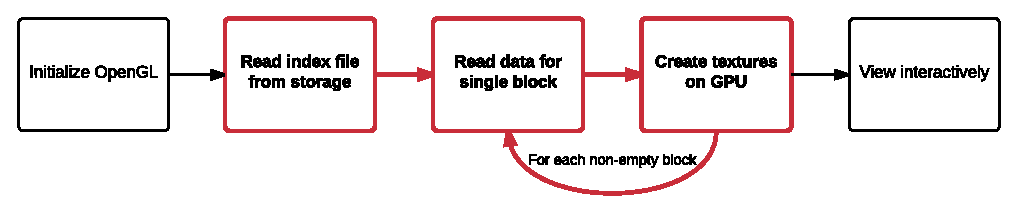
\includegraphics[width=\linewidth,height=0.3\textheight,keepaspectratio]{init-to-view-with-index-file}
		\caption{Volume visualization pipeline using the index file produced during preprocessing.}
	\end{centering}
\end{figure}

\paragraph{Proxy Geometry Creation for Each Subvolume}
In a traditional slice-based renderer, a set of 2D slices are used to resample the volume
texture at regularly space intervals. The number of slices depends on the sampling
rate used when collecting the volume data \cite{Engel2004}. The subvolume blocking approach 
requires a separate set of slice geometry for each 
subvolume. The number of slices per subvolume depends on the number of 
data samples within each subvolume and the number of subvolumes generated. In practice,
we choose to render each subvolume with a number of slices such that the total slices along
the current major axis is equal to the number of slices that would be used if rendering the 
dataset as a single large volume.

The basic approach does not reduce the size of the data on the GPU, but does
improve cache performance if the subvolumes are sized according to texture
cache size. In order to reduce the amount of data sent to the GPU we must have 
a way to determine which subvolumes are relevant to the visualization through
a classification process.

\begin{figure}[htb]\label{fig:volumeToSubvolumes}
	\begin{centering}
		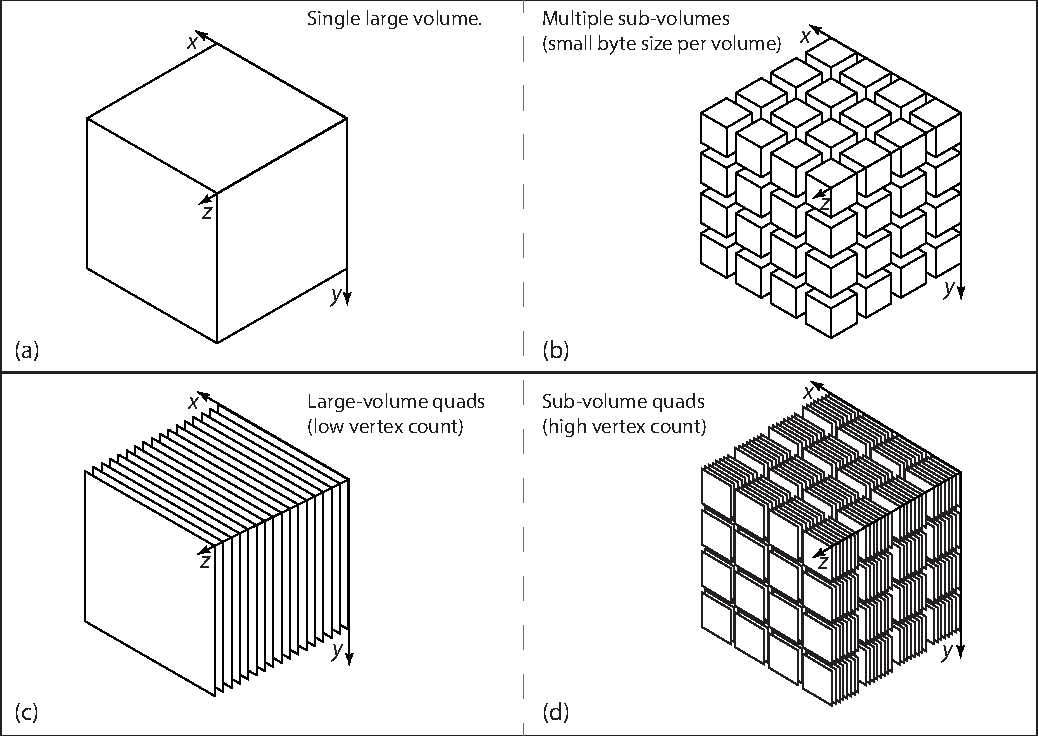
\includegraphics[width=\linewidth,height=0.3\textheight,keepaspectratio]{volume_to_subvolumes_and_quads}
		\caption{Initialization to view with partitioning.}
	\end{centering}
\end{figure}

\begin{algorithm}[]  
	\begin{algorithmic}[1]
		\Procedure{InitGpuTexture}{i, j, k, V} 
		\State $T_{i,j,k} \gets $ \Call{alloc}{$S_x \times S_y \times S_z$} \Comment{Allocate tex buffer}
		\For{$s_w \gets 0 .. S_z$} \Comment{For each voxel in $S_{i,j,k}$}
		\For{$s_v \gets 0 .. S_y$}
		\For{$s_u \gets 0 .. S_x$} 
		\State $u \gets s_u + i \times S_x$ \Comment{Compute offsets into V}
		\State $v \gets s_v + j \times S_y$ 
		\State $w \gets s_w + k \times S_z$ 
		\State $T_{i,j,k}\left[s_u, s_v, s_w \right] \gets V\left[u,v,w\right]$ \Comment{Copy to texture buffer}
		\EndFor
		\EndFor
		\EndFor
		\EndProcedure
	\end{algorithmic}
	\caption{Initialize texture $T_{i,j,k}$ for subvolume $S_{i,j,k}$.}
	\label{alg:initGpuTexture}
\end{algorithm}


\subsection{Subvolume blocking with classification}\label{sec:subvolumeBlockingWithClassification}

To facilitate easy data removal we extent the basic subvolume blocking approach
to include a classification step that identifies subvolumes relevant
to the desired visualization.  \textit{Relevant} subvolumes are expected to
contribute in some way to the visualization, otherwise a subvolume is
\textit{irrelevant}. Algorithm~\ref{alg:partitionAndThreshold} shows how the
classification step is merged  with the basic subdivision algorithm
(Algorithm~\ref{alg:initGpuTexture}).

Determining if a subvolume is relevant requires examining each voxel in the
subvolume to determine the voxel relevance. This per-voxel evaluation is done 
during a preprocessing step which generates an index file associating subvolumes
with subvolume statistics. At render time the index file is read and subvolumes are
classified as relevent or not based on the index file and a user supplied classifier
function, the minimum relevance threshold, and a total voxel
threshold. If the number of relevant voxels in the subvolume is above the total
relevant voxel threshold then the subvolume is relevant to the visualization.
Algorithm~\ref{alg:threasholdSubVolume} shows one way to determine subvolume
relevance from a voxel classifier ($C_{r}$), classification threshold ($t_{min}$),
and the relevant voxel threshold ($s_{min}$).

\begin{algorithm}[]
	\begin{algorithmic}[1]  
		\Procedure{PartitionAndThreshold}{$V$}
		\For{$i\gets 0 .. N_x$} \Comment{For each subvolume}  
		\For{$j\gets 0 .. N_y$}   
		\For{$k\gets 0 .. N_z$}   
		\If{\textit{subvolume i,j,k is relevant}} 
		\State \Call{InitGpuTexture}{i, j, k, V} \Comment{Send to GPU}
		\EndIf
		\EndFor
		\EndFor
		\EndFor
		\EndProcedure
	\end{algorithmic}
	\caption{Partition $V$ into subvolumes with thresholding.}
	\label{alg:partitionAndThreshold}
\end{algorithm}



\begin{algorithm}[]
	\begin{algorithmic}[1]
		\Procedure{IsSubvolumeRelevant}{$S_{i,j,k}, C_{r}, t_{min}, s_{min}$}
		\State $sum \gets 0$  \Comment{Relevant voxels found so far.}
		
		\ForAll{voxels in $S_{i,j,k}$}
		
		\State $r \gets$ \textit{voxel relevance from $C_{r}$} \Comment{Run classifier on voxel.}
		\If{\textit{$r > t_{min}$}} 
		\State $sum \gets sum + 1$  \Comment{Voxel is relevant}
		\EndIf
		\EndFor
		
		\If{\textit{$sum > s_{min}$}}
		\State \Return true \Comment{$S_{i,j,k}$ is relevant}
		\Else
		\State \Return false \Comment{$S_{i,j,k}$ is irrelevant}
		\EndIf
		\EndProcedure
	\end{algorithmic}
	\caption{Determine if $S_{i,j,k}$ is relevant to the visualization. $C_r$ is the classifier function,
		$t_{\min}$ is the classification threshold, and $s_{\min}$ is the relevant voxel threshold.}
	\label{alg:threasholdSubVolume}
\end{algorithm}

%\paragraph{Rejected Ejector Seat Reservation}
\section{Results}
Using our simple subvolume-based data reduction approach we are able to remove on average 80\% of
data from our test volumes and still maintain high-quality visualizations that run at interactive framerates. 
Our selected test volumes show that the usefulness of our technique is not limited to sparse volumes, but
any volumes with homogeneous regions of neighboring voxels. Because the classifier
function is user supplied the technique is flexible and can be tailored to the specific data set.

\begin{table}[h]
	\caption{Data reduction results.}\label{table:dataReduction}
	\scriptsize
	
	\begin{center}
		
		\begin{tabular}{lccc|cc}
			\textbf{Data set} & \textbf{Dimensions} & \textbf{Original Bytes} & \textbf{Block Dim} & \textbf{\% removal} & \textbf{Resulting Bytes} \\
			
			\hline
			
			Hop flower  (512)  &  $467x504x545$     &  $134$MB       & $16x16x16$    & 67\% &  $41$MB \\
	        Hop flower  (512)  &  $467x504x545$     &  $134$MB       & $32x32x32$   &  73\% & $34$MB \\
	        
	        Bone fragment (2.5K)  &  $2391x3084x2452$  & $18.0$GB    & $16x16x16$GB   & \% rem &  $00$ MB \\
			Bone fragment (2.5K)  &  $2391x3084x2452$  & $18.0$GB    & $32x32x32$GB    & \% rem &  $00$ MB \\

			Terrashake (2K)&  $XxYxZ$  & $0.0$GB    & $many$GB  & \% rem &  $00$ MB \\
			Terrashake (2K)&  $XxYxZ$  & $0.0$GB    & $many$GB  & \% rem &  $00$ MB \\

			Hop flower (4K) & $3509x3787x4096$   & $54.4$GB     & $16x16x16$     & 71\%    & $16$GB \\
			Hop flower (4K) & $3509x3787x4096$   & $54.4$GB      & $32x32x32$   & 75\%    & $13$GB \\

			Synthetic          &  $8\textnormal{K}^3$  & $549,755$M & $2.2$TB        & \% rem &  $00$ MB \\
		\end{tabular}
		
	\end{center}
	
\end{table}


\begin{table}[h]
	\caption{Cache performance}\label{table:cachePerformance}
	\scriptsize
	
	\begin{center}
		
		\begin{tabular}{lcccc|cccc}
			\textbf{Data set} & \textbf{Original Dim}& \textbf{Original Voxels} & \textbf{Original Size}& \textbf{Cache perf} & 
				\textbf{Voxels Removed} & \textbf{Block Size} & \textbf{\% removal} & \textbf{Cache perf}\\
			
			\hline
			
			Hop flower        & $512^3$                    &  $134$M       & $536$MB & cacheperf & vox rem & blockdim & \% rem & cacheperf \\
			Graphite foam   & $1\textnormal{K}^3$  & $1,073$M     & $4.3$GB & cacheperf & vox rem & blockdim & \% rem & cacheperf \\
			Bone fragment  & $2\textnormal{K}^3$  & $8,589$M    & $34.4$GB & cacheperf & vox rem  & blockdim & \% rem & cacheperf \\
			4K Hope flower & $4\textnormal{K}^3$  & $68,719$M   & $274.8$GB & cacheperf & vox rem & blockdim & \% rem & cacheperf \\
			Synthetic          & $8\textnormal{K}^3$  & $549,755$M & $2.2$TB & cacheperf & vox rem & blockdim & \% rem & cacheperf \\
		\end{tabular}
		
	\end{center}
	
\end{table}


\section{Conclusion}

%% if specified like this the section will be committed in review mode
\acknowledgments{}

\bibliographystyle{abbrv}
%%use following if all content of bibtex file should be shown
%\nocite{*}
\bibliography{template}
\end{document}
